% Options for packages loaded elsewhere
\PassOptionsToPackage{unicode}{hyperref}
\PassOptionsToPackage{hyphens}{url}
%
\documentclass[
]{article}
\usepackage{amsmath,amssymb}
\usepackage{lmodern}
\usepackage{iftex}
\ifPDFTeX
  \usepackage[T1]{fontenc}
  \usepackage[utf8]{inputenc}
  \usepackage{textcomp} % provide euro and other symbols
\else % if luatex or xetex
  \usepackage{unicode-math}
  \defaultfontfeatures{Scale=MatchLowercase}
  \defaultfontfeatures[\rmfamily]{Ligatures=TeX,Scale=1}
\fi
% Use upquote if available, for straight quotes in verbatim environments
\IfFileExists{upquote.sty}{\usepackage{upquote}}{}
\IfFileExists{microtype.sty}{% use microtype if available
  \usepackage[]{microtype}
  \UseMicrotypeSet[protrusion]{basicmath} % disable protrusion for tt fonts
}{}
\makeatletter
\@ifundefined{KOMAClassName}{% if non-KOMA class
  \IfFileExists{parskip.sty}{%
    \usepackage{parskip}
  }{% else
    \setlength{\parindent}{0pt}
    \setlength{\parskip}{6pt plus 2pt minus 1pt}}
}{% if KOMA class
  \KOMAoptions{parskip=half}}
\makeatother
\usepackage{xcolor}
\IfFileExists{xurl.sty}{\usepackage{xurl}}{} % add URL line breaks if available
\IfFileExists{bookmark.sty}{\usepackage{bookmark}}{\usepackage{hyperref}}
\hypersetup{
  hidelinks,
  pdfcreator={LaTeX via pandoc}}
\urlstyle{same} % disable monospaced font for URLs
\usepackage[margin=1in]{geometry}
\usepackage{color}
\usepackage{fancyvrb}
\newcommand{\VerbBar}{|}
\newcommand{\VERB}{\Verb[commandchars=\\\{\}]}
\DefineVerbatimEnvironment{Highlighting}{Verbatim}{commandchars=\\\{\}}
% Add ',fontsize=\small' for more characters per line
\usepackage{framed}
\definecolor{shadecolor}{RGB}{248,248,248}
\newenvironment{Shaded}{\begin{snugshade}}{\end{snugshade}}
\newcommand{\AlertTok}[1]{\textcolor[rgb]{0.94,0.16,0.16}{#1}}
\newcommand{\AnnotationTok}[1]{\textcolor[rgb]{0.56,0.35,0.01}{\textbf{\textit{#1}}}}
\newcommand{\AttributeTok}[1]{\textcolor[rgb]{0.77,0.63,0.00}{#1}}
\newcommand{\BaseNTok}[1]{\textcolor[rgb]{0.00,0.00,0.81}{#1}}
\newcommand{\BuiltInTok}[1]{#1}
\newcommand{\CharTok}[1]{\textcolor[rgb]{0.31,0.60,0.02}{#1}}
\newcommand{\CommentTok}[1]{\textcolor[rgb]{0.56,0.35,0.01}{\textit{#1}}}
\newcommand{\CommentVarTok}[1]{\textcolor[rgb]{0.56,0.35,0.01}{\textbf{\textit{#1}}}}
\newcommand{\ConstantTok}[1]{\textcolor[rgb]{0.00,0.00,0.00}{#1}}
\newcommand{\ControlFlowTok}[1]{\textcolor[rgb]{0.13,0.29,0.53}{\textbf{#1}}}
\newcommand{\DataTypeTok}[1]{\textcolor[rgb]{0.13,0.29,0.53}{#1}}
\newcommand{\DecValTok}[1]{\textcolor[rgb]{0.00,0.00,0.81}{#1}}
\newcommand{\DocumentationTok}[1]{\textcolor[rgb]{0.56,0.35,0.01}{\textbf{\textit{#1}}}}
\newcommand{\ErrorTok}[1]{\textcolor[rgb]{0.64,0.00,0.00}{\textbf{#1}}}
\newcommand{\ExtensionTok}[1]{#1}
\newcommand{\FloatTok}[1]{\textcolor[rgb]{0.00,0.00,0.81}{#1}}
\newcommand{\FunctionTok}[1]{\textcolor[rgb]{0.00,0.00,0.00}{#1}}
\newcommand{\ImportTok}[1]{#1}
\newcommand{\InformationTok}[1]{\textcolor[rgb]{0.56,0.35,0.01}{\textbf{\textit{#1}}}}
\newcommand{\KeywordTok}[1]{\textcolor[rgb]{0.13,0.29,0.53}{\textbf{#1}}}
\newcommand{\NormalTok}[1]{#1}
\newcommand{\OperatorTok}[1]{\textcolor[rgb]{0.81,0.36,0.00}{\textbf{#1}}}
\newcommand{\OtherTok}[1]{\textcolor[rgb]{0.56,0.35,0.01}{#1}}
\newcommand{\PreprocessorTok}[1]{\textcolor[rgb]{0.56,0.35,0.01}{\textit{#1}}}
\newcommand{\RegionMarkerTok}[1]{#1}
\newcommand{\SpecialCharTok}[1]{\textcolor[rgb]{0.00,0.00,0.00}{#1}}
\newcommand{\SpecialStringTok}[1]{\textcolor[rgb]{0.31,0.60,0.02}{#1}}
\newcommand{\StringTok}[1]{\textcolor[rgb]{0.31,0.60,0.02}{#1}}
\newcommand{\VariableTok}[1]{\textcolor[rgb]{0.00,0.00,0.00}{#1}}
\newcommand{\VerbatimStringTok}[1]{\textcolor[rgb]{0.31,0.60,0.02}{#1}}
\newcommand{\WarningTok}[1]{\textcolor[rgb]{0.56,0.35,0.01}{\textbf{\textit{#1}}}}
\usepackage{longtable,booktabs,array}
\usepackage{calc} % for calculating minipage widths
% Correct order of tables after \paragraph or \subparagraph
\usepackage{etoolbox}
\makeatletter
\patchcmd\longtable{\par}{\if@noskipsec\mbox{}\fi\par}{}{}
\makeatother
% Allow footnotes in longtable head/foot
\IfFileExists{footnotehyper.sty}{\usepackage{footnotehyper}}{\usepackage{footnote}}
\makesavenoteenv{longtable}
\usepackage{graphicx}
\makeatletter
\def\maxwidth{\ifdim\Gin@nat@width>\linewidth\linewidth\else\Gin@nat@width\fi}
\def\maxheight{\ifdim\Gin@nat@height>\textheight\textheight\else\Gin@nat@height\fi}
\makeatother
% Scale images if necessary, so that they will not overflow the page
% margins by default, and it is still possible to overwrite the defaults
% using explicit options in \includegraphics[width, height, ...]{}
\setkeys{Gin}{width=\maxwidth,height=\maxheight,keepaspectratio}
% Set default figure placement to htbp
\makeatletter
\def\fps@figure{htbp}
\makeatother
\setlength{\emergencystretch}{3em} % prevent overfull lines
\providecommand{\tightlist}{%
  \setlength{\itemsep}{0pt}\setlength{\parskip}{0pt}}
\setcounter{secnumdepth}{-\maxdimen} % remove section numbering
\ifLuaTeX
  \usepackage{selnolig}  % disable illegal ligatures
\fi

\author{}
\date{\vspace{-2.5em}}

\begin{document}

\hypertarget{appendix-apuxe9ndices}{%
\section*{(APPENDIX) Apéndices}\label{appendix-apuxe9ndices}}
\addcontentsline{toc}{section}{(APPENDIX) Apéndices}

\hypertarget{suxedmbolos-abreviaturas-y-acruxf3nimos}{%
\section{Símbolos, abreviaturas y
acrónimos}\label{suxedmbolos-abreviaturas-y-acruxf3nimos}}

\hypertarget{acruxf3nimos}{%
\subsection{Acrónimos}\label{acruxf3nimos}}

\begin{longtable}[]{@{}ll@{}}
\toprule
Acrónimo & Descripción \\
\midrule
\endhead
SPC & Statistical Process Control \\
\bottomrule
\end{longtable}

\hypertarget{letras-griegas}{%
\subsection{Letras griegas}\label{letras-griegas}}

\begin{longtable}[]{@{}ll@{}}
\toprule
Letra & Se lee \\
\midrule
\endhead
\(\alpha\) & alfa \\
\(\beta\) & beta \\
\(\gamma\) & gamma \\
\(\Gamma\) & Gamma\(^*\) \\
\(\lambda\) & lambda \\
\(\eta\) & eta \\
\(\mu\) & mu \\
\(\omega\) & omega \\
\(\Omega\) & Omega\(^*\) \\
\(\sigma\) & sigma \\
\(\Sigma\) & Sigma\(^*\) \\
\(\rho\) & ro \\
\(\theta\) & zeta (\emph{theta}, teta) \\
\(\xi\) & xi \\
\(\chi\) & chi (o \emph{ji}) \\
\(\pi\) & pi \\
\(\varepsilon\) & épsilon \\
\bottomrule
\end{longtable}

\(^*\) Mayúsculas

\hypertarget{suxedmbolos}{%
\subsection{Símbolos}\label{suxedmbolos}}

\begin{longtable}[]{@{}
  >{\raggedright\arraybackslash}p{(\columnwidth - 2\tabcolsep) * \real{0.4655}}
  >{\raggedright\arraybackslash}p{(\columnwidth - 2\tabcolsep) * \real{0.5345}}@{}}
\toprule
\begin{minipage}[b]{\linewidth}\raggedright
Símbolo
\end{minipage} & \begin{minipage}[b]{\linewidth}\raggedright
Se lee
\end{minipage} \\
\midrule
\endhead
\(\emptyset\) & Conjunto vacío o suceso imposible \\
\(\aleph\) & Aleph \\
\(\wp\) & Probabilidad (como función) \\
\(:\) & Tal que \\
\(P(\cdot)\) & Probabilidad de · (sucesos) \\
\(P[\cdot]\) & Probabilidad de · (variables aleatorias) \\
\(E[\cdot]\) & Esperanza de · \\
\(\cdot\) & \emph{lo que sea} (representa cualquier objeto
matemático) \\
\(|\) & Condicionado a \\
\(\sum\) & Sumatorio \\
\(\sum\limits_{i=1}^n\) & Sumatorio desde \(i\) igual a uno hasta
\(n\) \\
\(\prod\) & Producto \\
\(\prod\limits_{i=1}^n\) & Producto desde \(i\) igual a uno hasta
\(n\) \\
\(\forall\) & Para todo \\
\(\in\) & Pertenece/perteneciente \\
\(\exists\) & Existe \\
\(\implies\) & Implica/entonces \\
\(\partial\) & Derivada parcial \\
\(\simeq\) & Aproximadamente igual\footnote{En este libro se usa sobre
  todo para indicar que se ha redondeado un número decimal} \\
\(\approx\) & Aproximadamente\footnote{En este libro se puede utilizar
  para tomar el entero superior o inferior según el contexto} \\
\(\equiv\) & Equivalente \\
\(\mathbb{R}\) & Conjunto de los números reales \\
\(\cup\) & Unión \\
\(\cap\) & Intersección \\
\(\subset\) & Incluido \\
\(\subseteq\) & Incluido o igual \\
\bottomrule
\end{longtable}

\hypertarget{formulario}{%
\section{Formulario}\label{formulario}}

\hypertarget{estaduxedstica-descriptiva-univariante}{%
\subsection{Estadística descriptiva
univariante}\label{estaduxedstica-descriptiva-univariante}}

\hypertarget{notaciuxf3n}{%
\subsubsection{Notación}\label{notaciuxf3n}}

\begin{itemize}
\item
  \(X, Y, ...\): Variables.
\item
  \(x_i\):

  \begin{itemize}
  \tightlist
  \item
    En datos individuales: Cada uno de los valores observados de la
    variable \(X\)
  \item
    En datos agrupados: Cada uno de los \(k\) posibles valores de la
    variable \(X\).
  \end{itemize}
\item
  \(n\): Número total de observaciones en la muestra.
\item
  \(N\): Número total de observaciones en la población.
\item
  \(n_i\): Número de observaciones en la clase \(i\).
\item
  \(c_i\): Marca de clase en datos agrupados por intervalos.
\item
  \(L_i, i = 0, ..., k\): Límites de los intervalos \((L_{i-1}, L_i]\).
\end{itemize}

\hypertarget{tablas-de-frecuencias}{%
\subsubsection{Tablas de frecuencias}\label{tablas-de-frecuencias}}

\begin{itemize}
\item
  \(n_i\): Frecuencia absoluta, número de observaciones en la clase
  \(i\).
\item
  \(f_i\): Frecuencia relativa. \(f_i = \frac{n_i}{n}\)
\item
  \(N_i\): Frecuencia absoluta acumulada.
  \(N_i = \sum\limits_{j=1}^{i}n_j\)
\item
  \(N_i\): Frecuencia relativa acumulada.
  \(F_i = \sum\limits_{j=1}^{i}f_j = \frac{N_i}{n}\)
\item
  Número de intervalos en variables continuas:

  \begin{itemize}
  \tightlist
  \item
    Si \(n \leq 100, k\approx\sqrt n\)
  \item
    Si \(n > 100, k\approx 1 + \log_2 n\)
  \end{itemize}
\item
  \(A\): amplitud de la variable. \(A = x_{max} - x_{min}\)
\item
  \(a_i\): Amplitud de la clase \(i\). \(a_i = A/k\)
\item
  \(c_i\): Marca de clase. \(c_i = \frac{L_{i-1} + L_{i}}{2}\)
\end{itemize}

\hypertarget{medidas-de-tendencia-central}{%
\subsubsection{Medidas de tendencia
central}\label{medidas-de-tendencia-central}}

\begin{itemize}
\item
  Media aritmética: \(\bar{x}= \frac{\sum\limits_{i=1}^n x_i}{n}\).

  \begin{itemize}
  \tightlist
  \item
    Propiedad: \(Y = a+ bX \implies \bar y = a + b \bar x\)
  \item
    En variables discretas agrupadas:
    \(\bar{x}= \frac{1}{n}\sum\limits_{i=1}^k n_i x_i= \sum\limits_{i=1}^k f_i x_i,\)
  \item
    En variables agrupadas en intervalos:
    \(\bar{x}= \frac{1}{n}\sum\limits_{i=1}^k n_i c_i= \sum\limits_{i=1}^k f_i c_i\)
  \end{itemize}
\item
  Mediana: \(\min\limits_{i=1,...n}{x_i}: F_i\geq 0{,}5\)
\item
  Media geométrica:
  \(m_g = \left ( \Pi_{i=1}^n x_i\right)^{\frac{1}{n}}\)
\item
  Media armónica: \(H = \frac{n}{\sum\limits_{i=1}^n\frac{ 1}{ x_i}}\)
\end{itemize}

\hypertarget{medidas-de-posiciuxf3n} = \min\limits_{i=1,...n}{x_i}: F_i\geq p/ 100\)
\item
  Cuartiles: \(Q_1 = P_{25}\); \(Q_3 = P_{75}\)
\end{itemize}

\hypertarget{medidas-de-dispersiuxf3n}{%
\subsubsection{Medidas de dispersión}\label{medidas-de-dispersiuxf3n}}

\begin{itemize}
\item
  Rango o recorrido: \(R = \max\limits_i{x_i} - \min\limits_i{x_i}\)
\item
  Desviación media absoluta:
  \(\mathit{DMA} = \frac{1}{n}\sum\limits_{i=1}^n |x_i-\bar x|.\)
\item
  Desviación absoluta mediana:
  \(\mathit{DAM} = Me |x_i- Me_x|,\; i = 1, \ldots, n.\)
\item
  Varianza muestral o cuasivarianza:
  \(s^2= \frac{\sum\limits_{i=1}^n (x_i- \bar{x})^2}{n-1} = \frac{1}{n-1}\left (\sum\limits_{i=1}^n x_i^2 - n \bar x^2\right )\)
\item
  Varianza poblacional:
  \(\sigma^2= \frac{\sum\limits_{i=1}^N (X_i- \mu)^2}{N} = \frac{1}{N} \sum\limits_{i=1}^n X_i^2 - \mu^2\)
\item
  Desviación típica muestral o cuasidesviación típica:
  \(s= \sqrt{s^2} = \sqrt{\frac{\sum\limits_{i=1}^n (x_i- \bar{x})^2}{n-1}}\).
\item
  Propiedad de la varianza: \(Y=a+bX \implies s_y^2=b^2s^2_X\)
\item
  Tipificación: \(Z = \frac{X-\bar x}{s} \implies \bar z = 0; s^2 = 1\)
\item
  Coeficiente de variación: \(\mathit{CV} = \frac{s}{|\bar x|}\)
\item
  Rango intercuartílico: \(IQR = Q_3 - Q_1\)
\end{itemize}

\hypertarget{medidas-de-forma}{%
\subsubsection{Medidas de forma}\label{medidas-de-forma}}

\begin{itemize}
\tightlist
\item
  Coeficiente de asimetría: \(\gamma_1 = \frac{m_3}{s^3}\)

  \begin{itemize}
  \tightlist
  \item
    \(m_3 = \frac{1}{n}\sum\limits_{i=1}^n(x-\bar x ) ^3\)
  \end{itemize}
\item
  Coeficiente de curtosis (apuntamiento):
  \(\gamma_2 = \frac{m_4}{s^4}-3\)

  \begin{itemize}
  \tightlist
  \item
    \(m_4 = \frac{1}{n}\sum\limits_{i=1}^n(x-\bar x ) ^4\)
  \end{itemize}
\end{itemize}

\hypertarget{estaduxedstica-descriptiva-bivariante}{%
\subsection{Estadística descriptiva
bivariante}\label{estaduxedstica-descriptiva-bivariante}}

\hypertarget{notaciuxf3n-1}{%
\subsubsection{Notación}\label{notaciuxf3n-1}}

\begin{itemize}
\item
  \(X, Y, ...\): Variables.
\item
  \(x_i\), \(y_j\): Cada uno de los \(k\) posibles valores de la
  variable \(X\).
\item
  \((x_i, y_i)\): Cada uno de los \(n\) pares de valores observados.
\item
  \(n\): Número total de observaciones en la muestra.
\item
  \(n_i\): Número de clases de la variable \(X\).
\item
  \(n_j\): Número de clases de la variable \(Y\).
\item
  \(n_{ij}\): Número de observaciones en la clase \(i\) de la variable
  \(X\) \textbf{y} en la clase \(j\) de la variable \(Y\).
\end{itemize}

\hypertarget{tablas-de-frecuencias-1}{%
\subsubsection{Tablas de frecuencias}\label{tablas-de-frecuencias-1}}

\begin{itemize}
\item
  \(n_{ij}\): Frecuencia absoluta conjunta, número de observaciones en
  la clase \(i\) de la variable \(X\) \textbf{y} en la clase \(j\) de la
  variable \(Y\).
\item
  \(f_{ij}\): Frecuencia relativa conjunta.
  \(f_{ij} = \frac{n_{ij}}{n}\)
\item
  Frecuencias marginales de \(X\):

  \begin{itemize}
  \tightlist
  \item
    Absolutas: \(n_{i\cdot} = \sum\limits_{j = 1}^{n_j}n_{ij}\)
  \item
    Relativas: \(f_{i\cdot} = \sum\limits_{j = 1}^{n_j}f_{ij}\)
  \end{itemize}
\item
  Frecuencias marginales de \(Y\):

  \begin{itemize}
  \tightlist
  \item
    \(n_{\cdot j} = \sum\limits_{i = 1}^{n_i}n_{ij}\)
  \item
    \(f_{\cdot j} = \sum\limits_{i = 1}^{n_i}f_{ij}\)
  \end{itemize}
\item
  Frecuencias condicionadas:

  \begin{itemize}
  \tightlist
  \item
    \(f_{x_i|y=y_j}=\frac{n_{ij}}{n_{·j}}.\)
  \item
    \(f_{y_j|x=x_y}=\frac{n_{ij}}{n_{i·}}.\)
  \end{itemize}
\item
  Independencia: Si \(f_{ij} = f_{i.}\cdot f_{.j} \;\forall i, j\),
  entonces las variables \(X\) e \(Y\) son independientes.
\end{itemize}

\hypertarget{covarianza-y-correlaciuxf3n}{%
\subsubsection{Covarianza y
correlación}\label{covarianza-y-correlaciuxf3n}}

\begin{itemize}
\item
  Covarianza poblacional:

  \begin{itemize}
  \tightlist
  \item
    Definición:
    \(\sigma_{xy} = \frac{1}{N} \sum\limits_{i=1}^n(X_i-\bar X)(Y_i-\bar Y)\)
  \item
    Cálculo abreviado:
    \(\sigma_{xy} = \frac{1}{N} \sum\limits_{i=1}^N(X_i \cdot Y_i) - \bar X \cdot \bar Y\)
  \end{itemize}
\item
  Covarianza muestral:

  \begin{itemize}
  \tightlist
  \item
    Definición:
    \(s_{xy} = \frac{1}{n-1} \sum\limits_{i=1}^n(x_i-\bar x)(y_i-\bar y)\)
  \item
    Cálculo abreviado:
    \(s_{xy} = \frac{1}{n-1} \left ( \sum\limits_{i=1}^n(x_i \cdot y_i) - n \cdot \bar x \cdot \bar y \right )\)
  \end{itemize}
\item
  Coeficiente de correlación lineal:
  \(r_{xy}=\frac{s_{xy}}{s_x \cdot s_y}\)
\item
  Matriz de covarianzas (caso bivariante):
\end{itemize}

\[\mathbf{S} = \left [\begin{array}{cc}
s^2_x & s_{xy}\\
s_{xy} & s_y^2
\end{array}\right ]\]

\hypertarget{regresiuxf3n-lineal-simple}{%
\subsubsection{Regresión lineal
simple}\label{regresiuxf3n-lineal-simple}}

\begin{itemize}
\item
  Recta de regresión: \(y=a+bx\)

  \begin{itemize}
  \tightlist
  \item
    \(b = \frac{s_{xy}}{s_x^2}\)
  \item
    \(a = \bar y - b \bar x\)
  \item
    \(b = \frac{s_y}{s_x}r_{xy}\)
  \end{itemize}
\item
  Predicción de nuevos valores: \(\hat{y}_{n+1} = a + bx_{n+1}\)
\item
  Residuos: \(\varepsilon_i=y_i - \hat{y}_i = y_i - (a+bx_i)\)
\item
  Varianza residual:
  \(s_\varepsilon^2= \frac{1}{n}\sum\limits_{i=1}^n \varepsilon_i^2\)

  \begin{itemize}
  \tightlist
  \item
    \(\frac{s_\varepsilon^2}{s_y^2}=(1-r_{xy}^2)\)
  \end{itemize}
\item
  Coeficiente de determinación:
  \(R^2 = 1- \frac{s_\varepsilon^2}{s_y^2} = r^2_{xy}\)
\end{itemize}

\hypertarget{probabilidad}{%
\subsection{Probabilidad}\label{probabilidad}}

\hypertarget{notaciuxf3n-2}{%
\subsubsection{Notación}\label{notaciuxf3n-2}}

\begin{itemize}
\tightlist
\item
  \(A, B, \ldots\): Sucesos
\item
  \(\omega\): Suceso elemental
\item
  \(\Omega\): Espacio muestral
\item
  \(\emptyset\): Suceso imposible
\item
  \(A^c\): Suceso complementario del suceso \(A\)
\end{itemize}

\hypertarget{definiciones}{%
\subsubsection{Definiciones}\label{definiciones}}

\begin{itemize}
\tightlist
\item
  Unión de sucesos: \(A \cup B\): Ocurre \(A\) \textbf{o} Ocurre \(B\),
  o los dos
\item
  Intersección de sucesos: \(A \cap B\): Ocurre \(A\) \textbf{y} Ocurre
  \(B\)
\item
  Sucesos disjuntos o mutuamente excluyentes, o incompatibles:
  \(A \cap B = \emptyset\)
\item
  Partición del espacio muestral: Colección de sucesos
  \(A_1, A_2, \ldots \in \Omega\) que cumplen:

  \begin{itemize}
  \tightlist
  \item
    \(A_1, A_2, \ldots: \quad A_i \subset \Omega \; \forall i\)
  \item
    \(A_i \cap A_j = \emptyset \; \forall i \neq j\),
  \item
    \(\displaystyle \underset{i}\bigcup A_i = \Omega\).
  \end{itemize}
\item
  Sigma álgebra de sucesos \(\aleph\) (\emph{aleph}). conjunto de
  sucesos que:

  \begin{itemize}
  \tightlist
  \item
    Pertenecen a \(\aleph\),
  \item
    Si \(A \in \aleph \implies A^c \in \aleph\)
  \item
    Si \(\{A_i\}\in \aleph\;\; \forall i\), entonces
    \(\displaystyle \underset{i}\bigcup A_i \in \aleph\) y
    \(\displaystyle \underset{i}\bigcap A_i \in \aleph\)
  \end{itemize}
\end{itemize}

\hypertarget{propiedades}{%
\subsubsection{Propiedades}\label{propiedades}}

\begin{itemize}
\tightlist
\item
  \textbf{Conmutativa}:

  \begin{itemize}
  \tightlist
  \item
    \(A\cup B= B\cup A\).
  \item
    \(A\cap B= B\cap A\).
  \end{itemize}
\item
  \textbf{Asociativa}:

  \begin{itemize}
  \tightlist
  \item
    \(A \cup (B \cup C) = (A \cup B) \cup C\).
  \item
    \(A \cap (B \cap C) = (A \cap B) \cap C\).
  \end{itemize}
\item
  \textbf{Distributiva}:

  \begin{itemize}
  \tightlist
  \item
    \(A \cup (B \cap C) = (A \cup B) \cap (A \cup C)\).
  \item
    \(A \cap (B \cup C) = (A \cap B) \cup (A \cap C)\).
  \end{itemize}
\item
  \textbf{Leyes de De Morgan}:

  \begin{itemize}
  \tightlist
  \item
    \((A \cup B)^c = A^c \cap B^c\).
  \item
    \((A \cap B)^c = A^c \cup B^c\).
  \end{itemize}
\item
  \(A \cup A = A \cap A = A \cup \emptyset = A \cap \Omega = A\).
\item
  \(A \cup \Omega = \Omega\).
\end{itemize}

\hypertarget{definiciones-de-probabilidad}{%
\subsection{Definiciones de
probabilidad}\label{definiciones-de-probabilidad}}

\begin{itemize}
\item
  Definición de Laplace:
  \(P(A) = \frac{\text{casos favorables a } A}{\text{casos posibles}}\)
\item
  Definición frecuentista:
  \(P(A) = \lim\limits_{n \to \infty} \frac{n(A)}{n}\)
\item
  Definición axiomática:

  \begin{itemize}
  \tightlist
  \item
    \textbf{Primer axioma}:
    \(\forall A \in \aleph \; \exists \; P(A) \geq 0\).
  \item
    \textbf{Segundo axioma}: \(P(\Omega) = 1\).
  \item
    \textbf{Tercer axioma}: Dada la sucesión
    \(A_1, \ldots, A_i, \ldots: A_i \in \aleph \; \forall\, i, A_i \cap A_j = \emptyset \; \forall i \neq j\),
    se cumple:
  \end{itemize}
\end{itemize}

\[P \left (\bigcup\limits_{i=1}^{\infty} A_i \right ) = \sum\limits_{i=1}^{\infty} P(A_i).\]

\hypertarget{teoremas-derivados}{%
\subsubsection{Teoremas derivados}\label{teoremas-derivados}}

\begin{itemize}
\tightlist
\item
  Dados \(n\) sucesos disjuntos dos a dos
  \(A_1, \ldots, A_n: A_i \cap A_j = \emptyset \; \forall i \neq j\):
\end{itemize}

\[P \left (\bigcup\limits_{i=1}^{n} A_i \right ) = \sum\limits_{i=1}^{n} P(A_i).\]
* \(P(A^c)=1-P(A)\).

\begin{itemize}
\item
  \(P(\emptyset) = 0\).
\item
  Dados \(A_1, A_2: A_1 \subset A_2 \implies P(A_1) \leq P(A_2)\).
\item
  \(P(A \cup B) = P(A) + P(B) - P(A \cap B)\).
\item
  \(P(\bigcup\limits_{i=1}^n A_i) = \sum\limits_{i=1}^n P(A_i) - \sum\limits_{i<j} P(A_i \cap A_j) + \sum\limits_{i<j<k} P(A_i \cap A_j \cap A_k) -\)\\
  \(- \ldots + (-1)^{n-1} P \left(\bigcap\limits_{i=1}^n A_i\right ).\)
\end{itemize}

\[ \boxed{0 \leq P(A) \leq 1}.\]

\hypertarget{probabilidad-condicionada-e-independencia}{%
\subsubsection{Probabilidad condicionada e
independencia}\label{probabilidad-condicionada-e-independencia}}

\begin{itemize}
\tightlist
\item
  Probabilidad de \(A\) condicionada a \(B\):
  \({P(A | B)=\frac{P(A \cap B)}{P(B)}}\)
\item
  Probabilidad de la interesección:
  \(\boxed{P(A\cap B)=P(A|B)\cdot P(B)=P(B|A)\cdot P(A)}\)
\item
  Regla de la cadena:
  \[P\left( \bigcap\limits_{i=1}^{n} A_i \right) = P(A_1)\cdot P(A_2|A_1)\cdot P(A_3|A_1 \cap A_2)\cdot\ldots\cdot P\left(A_n | \bigcap\limits_{i=1}^{n-1} S_i \right)\]
\item
  \(A\) y \(B\) independientes
  \(\iff P(A|B) = P(A)\;\; \text{y}\;\; P(B|A) = P(B)\)

  \begin{itemize}
  \tightlist
  \item
    \(\boxed{P(A\cap B)=P(A)\cdot P(B)}\) (solo si son independientes)
  \item
    \(P(A^c|B) = 1- P(A^c|B)\)
  \end{itemize}
\end{itemize}

\hypertarget{probabilidad-total-y-fuxf3rmula-de-bayes}{%
\subsubsection{Probabilidad total y fórmula de
Bayes}\label{probabilidad-total-y-fuxf3rmula-de-bayes}}

\begin{itemize}
\tightlist
\item
  Probabilidad total:
\end{itemize}

\[\boxed{P(B)=\sum\limits_{i=1}^{n} P(B/A_i)\cdot P(A_i)}\]

\begin{itemize}
\tightlist
\item
  Fórmula de Bayes:
\end{itemize}

\[\boxed{P(A_i|B)=\frac{P(B|A_i)\cdot P(A_i)}{\sum\limits_{i=1}^{n} P(B/A_i)\cdot P(A_i)}}\]

\hypertarget{variable-aleatoria}{%
\subsection{Variable aleatoria}\label{variable-aleatoria}}

\hypertarget{inferencia}{%
\subsection{Inferencia}\label{inferencia}}

\hypertarget{calidad}{%
\subsection{Calidad}\label{calidad}}

\hypertarget{tablas}{%
\section{Tablas estadísticas}\label{tablas}}

\hypertarget{distribuciuxf3n-normal}{%
\subsection{Distribución normal}\label{distribuciuxf3n-normal}}

La siguiente tabla contiene la probabilidad de la cola inferior de la
distribución normal estándar \(Z\sim N(0;1)\), es decir
\(F(z)=P[Z\leq z].\).

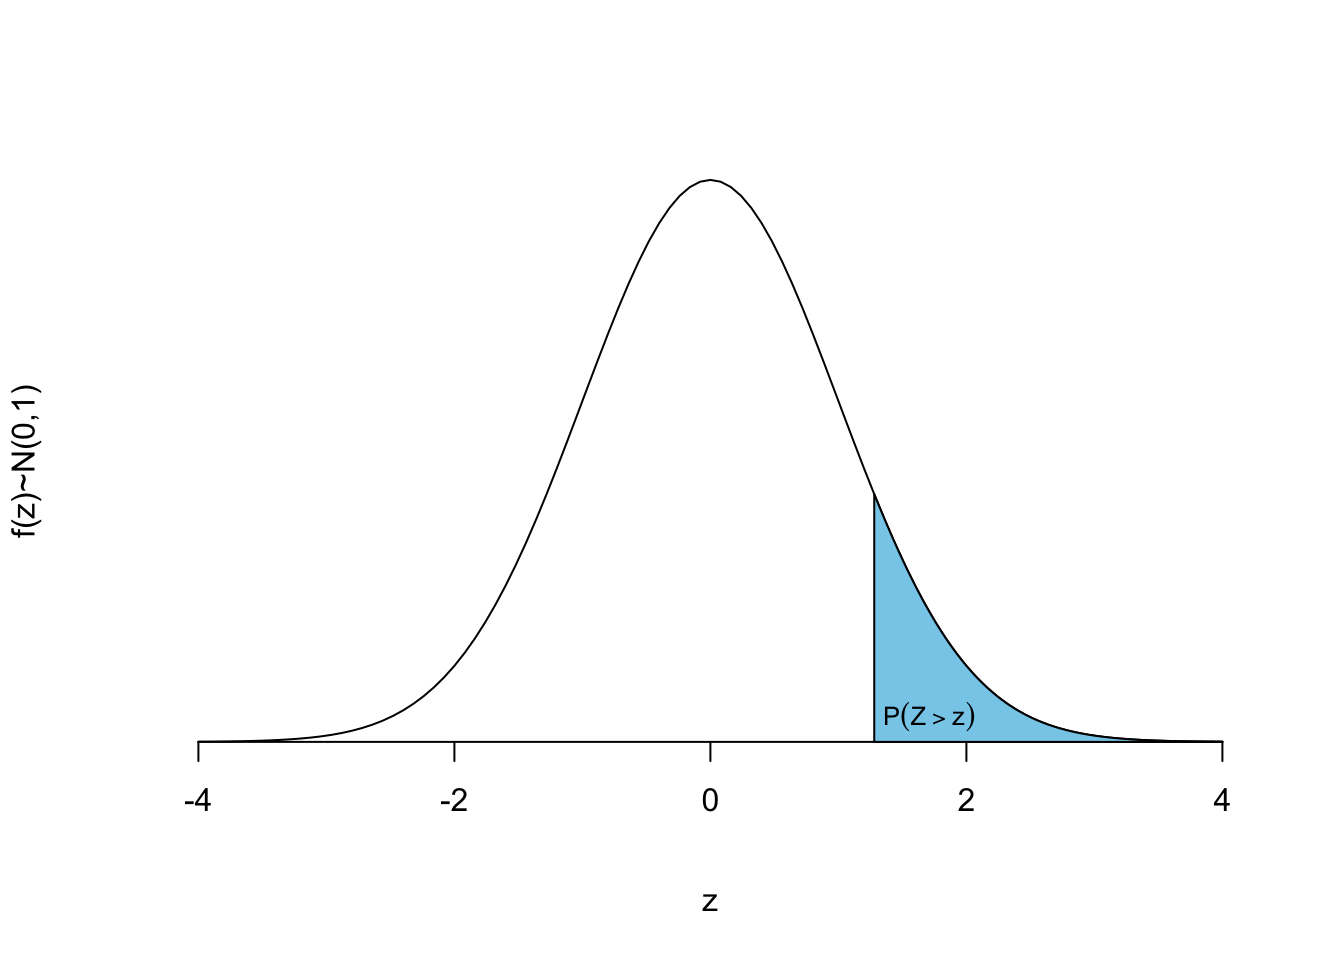
\includegraphics[width=0.7\linewidth]{91-apendices_files/figure-latex/unnamed-chunk-2-1}

\begin{longtable}[]{@{}
  >{\raggedleft\arraybackslash}p{(\columnwidth - 20\tabcolsep) * \real{0.0541}}
  >{\raggedleft\arraybackslash}p{(\columnwidth - 20\tabcolsep) * \real{0.0946}}
  >{\raggedleft\arraybackslash}p{(\columnwidth - 20\tabcolsep) * \real{0.0946}}
  >{\raggedleft\arraybackslash}p{(\columnwidth - 20\tabcolsep) * \real{0.0946}}
  >{\raggedleft\arraybackslash}p{(\columnwidth - 20\tabcolsep) * \real{0.0946}}
  >{\raggedleft\arraybackslash}p{(\columnwidth - 20\tabcolsep) * \real{0.0946}}
  >{\raggedleft\arraybackslash}p{(\columnwidth - 20\tabcolsep) * \real{0.0946}}
  >{\raggedleft\arraybackslash}p{(\columnwidth - 20\tabcolsep) * \real{0.0946}}
  >{\raggedleft\arraybackslash}p{(\columnwidth - 20\tabcolsep) * \real{0.0946}}
  >{\raggedleft\arraybackslash}p{(\columnwidth - 20\tabcolsep) * \real{0.0946}}
  >{\raggedleft\arraybackslash}p{(\columnwidth - 20\tabcolsep) * \real{0.0946}}@{}}
\toprule
\begin{minipage}[b]{\linewidth}\raggedleft
z
\end{minipage} & \begin{minipage}[b]{\linewidth}\raggedleft
0.00
\end{minipage} & \begin{minipage}[b]{\linewidth}\raggedleft
0.01
\end{minipage} & \begin{minipage}[b]{\linewidth}\raggedleft
0.02
\end{minipage} & \begin{minipage}[b]{\linewidth}\raggedleft
0.03
\end{minipage} & \begin{minipage}[b]{\linewidth}\raggedleft
0.04
\end{minipage} & \begin{minipage}[b]{\linewidth}\raggedleft
0.05
\end{minipage} & \begin{minipage}[b]{\linewidth}\raggedleft
0.06
\end{minipage} & \begin{minipage}[b]{\linewidth}\raggedleft
0.07
\end{minipage} & \begin{minipage}[b]{\linewidth}\raggedleft
0.08
\end{minipage} & \begin{minipage}[b]{\linewidth}\raggedleft
0.09
\end{minipage} \\
\midrule
\endhead
0.0 & 0.5000 & 0.5040 & 0.5080 & 0.5120 & 0.5160 & 0.5199 & 0.5239 &
0.5279 & 0.5319 & 0.5359 \\
0.1 & 0.5398 & 0.5438 & 0.5478 & 0.5517 & 0.5557 & 0.5596 & 0.5636 &
0.5675 & 0.5714 & 0.5753 \\
0.2 & 0.5793 & 0.5832 & 0.5871 & 0.5910 & 0.5948 & 0.5987 & 0.6026 &
0.6064 & 0.6103 & 0.6141 \\
0.3 & 0.6179 & 0.6217 & 0.6255 & 0.6293 & 0.6331 & 0.6368 & 0.6406 &
0.6443 & 0.6480 & 0.6517 \\
0.4 & 0.6554 & 0.6591 & 0.6628 & 0.6664 & 0.6700 & 0.6736 & 0.6772 &
0.6808 & 0.6844 & 0.6879 \\
0.5 & 0.6915 & 0.6950 & 0.6985 & 0.7019 & 0.7054 & 0.7088 & 0.7123 &
0.7157 & 0.7190 & 0.7224 \\
0.6 & 0.7257 & 0.7291 & 0.7324 & 0.7357 & 0.7389 & 0.7422 & 0.7454 &
0.7486 & 0.7517 & 0.7549 \\
0.7 & 0.7580 & 0.7611 & 0.7642 & 0.7673 & 0.7704 & 0.7734 & 0.7764 &
0.7794 & 0.7823 & 0.7852 \\
0.8 & 0.7881 & 0.7910 & 0.7939 & 0.7967 & 0.7995 & 0.8023 & 0.8051 &
0.8078 & 0.8106 & 0.8133 \\
0.9 & 0.8159 & 0.8186 & 0.8212 & 0.8238 & 0.8264 & 0.8289 & 0.8315 &
0.8340 & 0.8365 & 0.8389 \\
1.0 & 0.8413 & 0.8438 & 0.8461 & 0.8485 & 0.8508 & 0.8531 & 0.8554 &
0.8577 & 0.8599 & 0.8621 \\
1.1 & 0.8643 & 0.8665 & 0.8686 & 0.8708 & 0.8729 & 0.8749 & 0.8770 &
0.8790 & 0.8810 & 0.8830 \\
1.2 & 0.8849 & 0.8869 & 0.8888 & 0.8907 & 0.8925 & 0.8944 & 0.8962 &
0.8980 & 0.8997 & 0.9015 \\
1.3 & 0.9032 & 0.9049 & 0.9066 & 0.9082 & 0.9099 & 0.9115 & 0.9131 &
0.9147 & 0.9162 & 0.9177 \\
1.4 & 0.9192 & 0.9207 & 0.9222 & 0.9236 & 0.9251 & 0.9265 & 0.9279 &
0.9292 & 0.9306 & 0.9319 \\
1.5 & 0.9332 & 0.9345 & 0.9357 & 0.9370 & 0.9382 & 0.9394 & 0.9406 &
0.9418 & 0.9429 & 0.9441 \\
1.6 & 0.9452 & 0.9463 & 0.9474 & 0.9484 & 0.9495 & 0.9505 & 0.9515 &
0.9525 & 0.9535 & 0.9545 \\
1.7 & 0.9554 & 0.9564 & 0.9573 & 0.9582 & 0.9591 & 0.9599 & 0.9608 &
0.9616 & 0.9625 & 0.9633 \\
1.8 & 0.9641 & 0.9649 & 0.9656 & 0.9664 & 0.9671 & 0.9678 & 0.9686 &
0.9693 & 0.9699 & 0.9706 \\
1.9 & 0.9713 & 0.9719 & 0.9726 & 0.9732 & 0.9738 & 0.9744 & 0.9750 &
0.9756 & 0.9761 & 0.9767 \\
2.0 & 0.9772 & 0.9778 & 0.9783 & 0.9788 & 0.9793 & 0.9798 & 0.9803 &
0.9808 & 0.9812 & 0.9817 \\
2.1 & 0.9821 & 0.9826 & 0.9830 & 0.9834 & 0.9838 & 0.9842 & 0.9846 &
0.9850 & 0.9854 & 0.9857 \\
2.2 & 0.9861 & 0.9864 & 0.9868 & 0.9871 & 0.9875 & 0.9878 & 0.9881 &
0.9884 & 0.9887 & 0.9890 \\
2.3 & 0.9893 & 0.9896 & 0.9898 & 0.9901 & 0.9904 & 0.9906 & 0.9909 &
0.9911 & 0.9913 & 0.9916 \\
2.4 & 0.9918 & 0.9920 & 0.9922 & 0.9925 & 0.9927 & 0.9929 & 0.9931 &
0.9932 & 0.9934 & 0.9936 \\
2.5 & 0.9938 & 0.9940 & 0.9941 & 0.9943 & 0.9945 & 0.9946 & 0.9948 &
0.9949 & 0.9951 & 0.9952 \\
2.6 & 0.9953 & 0.9955 & 0.9956 & 0.9957 & 0.9959 & 0.9960 & 0.9961 &
0.9962 & 0.9963 & 0.9964 \\
2.7 & 0.9965 & 0.9966 & 0.9967 & 0.9968 & 0.9969 & 0.9970 & 0.9971 &
0.9972 & 0.9973 & 0.9974 \\
2.8 & 0.9974 & 0.9975 & 0.9976 & 0.9977 & 0.9977 & 0.9978 & 0.9979 &
0.9979 & 0.9980 & 0.9981 \\
2.9 & 0.9981 & 0.9982 & 0.9982 & 0.9983 & 0.9984 & 0.9984 & 0.9985 &
0.9985 & 0.9986 & 0.9986 \\
3.0 & 0.9987 & 0.9987 & 0.9987 & 0.9988 & 0.9988 & 0.9989 & 0.9989 &
0.9989 & 0.9990 & 0.9990 \\
3.1 & 0.9990 & 0.9991 & 0.9991 & 0.9991 & 0.9992 & 0.9992 & 0.9992 &
0.9992 & 0.9993 & 0.9993 \\
3.2 & 0.9993 & 0.9993 & 0.9994 & 0.9994 & 0.9994 & 0.9994 & 0.9994 &
0.9995 & 0.9995 & 0.9995 \\
3.3 & 0.9995 & 0.9995 & 0.9995 & 0.9996 & 0.9996 & 0.9996 & 0.9996 &
0.9996 & 0.9996 & 0.9997 \\
3.4 & 0.9997 & 0.9997 & 0.9997 & 0.9997 & 0.9997 & 0.9997 & 0.9997 &
0.9997 & 0.9997 & 0.9998 \\
3.5 & 0.9998 & 0.9998 & 0.9998 & 0.9998 & 0.9998 & 0.9998 & 0.9998 &
0.9998 & 0.9998 & 0.9998 \\
3.6 & 0.9998 & 0.9998 & 0.9999 & 0.9999 & 0.9999 & 0.9999 & 0.9999 &
0.9999 & 0.9999 & 0.9999 \\
3.7 & 0.9999 & 0.9999 & 0.9999 & 0.9999 & 0.9999 & 0.9999 & 0.9999 &
0.9999 & 0.9999 & 0.9999 \\
3.8 & 0.9999 & 0.9999 & 0.9999 & 0.9999 & 0.9999 & 0.9999 & 0.9999 &
0.9999 & 0.9999 & 0.9999 \\
3.9 & 1.0000 & 1.0000 & 1.0000 & 1.0000 & 1.0000 & 1.0000 & 1.0000 &
1.0000 & 1.0000 & 1.0000 \\
\bottomrule
\end{longtable}

\hypertarget{resumen-modelos-de-distribuciuxf3n-de-probabilidad}{%
\subsection{Resumen modelos de distribución de
probabilidad}\label{resumen-modelos-de-distribuciuxf3n-de-probabilidad}}

\begin{longtable}[]{@{}
  >{\raggedright\arraybackslash}p{(\columnwidth - 6\tabcolsep) * \real{0.2357}}
  >{\raggedright\arraybackslash}p{(\columnwidth - 6\tabcolsep) * \real{0.6433}}
  >{\raggedright\arraybackslash}p{(\columnwidth - 6\tabcolsep) * \real{0.0637}}
  >{\raggedright\arraybackslash}p{(\columnwidth - 6\tabcolsep) * \real{0.0573}}@{}}
\toprule
\begin{minipage}[b]{\linewidth}\raggedright
Distribución
\end{minipage} & \begin{minipage}[b]{\linewidth}\raggedright
Probabilidad/Densidad/Distribución
\end{minipage} & \begin{minipage}[b]{\linewidth}\raggedright
Esperanza
\end{minipage} & \begin{minipage}[b]{\linewidth}\raggedright
Varianza
\end{minipage} \\
\midrule
\endhead
\(\text{Bernoulli}\\ \mathit{Ber}(p)\) &
\(X = \begin{cases} 1 & \mbox{ con probabilidad } p \\ 0 & \mbox{ con probabilidad } 1-p \end{cases}\)
& \(p\) & \(p(1-p)\) \\
\bottomrule
\end{longtable}

\hypertarget{repaso}{%
\section{Repaso}\label{repaso}}

Este apéndice cubre algunas cuestiones matemáticas básicas que el lector
de este libro con seguridad habrá aprendido con anterioridad. Se
incluyen como referencia para facilitar el repaso a aquellos que lo
necesiten.

\hypertarget{logaritmos-y-exponenciales}{%
\subsection{Logaritmos y
exponenciales}\label{logaritmos-y-exponenciales}}

\hypertarget{combinatoria}{%
\subsection{Combinatoria}\label{combinatoria}}

Una de las definiciones de probabilidad implica \textbf{contar} el
número de veces que puede ocurrir un suceso determinado. Por tanto, en
muchas ocasiones el cálculo de probabilidades empieza contando las
posibilidades de que ocurra un suceso. La Combinatoria es la parte de la
Matemática discreta que nos ayuda en esta tarea. Incluimos un breve
resumen con ejemplos de las fórmulas más habituales y su cálculo con R.

\hypertarget{ejemplo-ilustrativo}{%
\subsubsection{Ejemplo ilustrativo}\label{ejemplo-ilustrativo}}

Habitualmente se utilizan ejemplos de juegos de azar para introducir el
cálculo de probabilidades, como lanzamiendo de monedas y dados, o
combinaciones de cartas en barajas de naipes. Para darle un enfoque
práctico, utilizaremos a lo largo del módulo un ejemplo ilustrativo que,
aunque totalmente inventado, se puede encontrar el lector en el futuro
con ligeras variaciones según su ámbito de actuación. Utilizaremos en lo
posible las cifras usadas en los problemas de azar para ver la utilidad
de aquéllos ejemplos en casos más prácticos.

Datos básicos:

\begin{itemize}
\item
  52 posibles usuarios de un servicio
\item
  La mitad son mujeres
\item
  4 directivos, 12 mandos, resto operarios
\item
  13 jóvenes, 26 adultos, 13 mayores (5, 18 y 3 mujeres en cada grupo
  respectivamente)
\item
  1 de cada seis hombres contratará el servicio (el doble si es mujer)
\end{itemize}

Nótese cómo podemos \emph{traducir} el concepto de servicio a cualquier
ámbito: usuarios de salud o educación, enfermos de una determinada
patología, equipos de una infraestructura, etc. Asimismo las categorías
pueden ser cualesquiera aplicables a los elementos de los conjuntos.

\hypertarget{principio-buxe1sico-de-conteo}{%
\subsubsection{Principio básico de
conteo}\label{principio-buxe1sico-de-conteo}}

\textbf{Definición}: Realizamos \(k\) experimentos sucesivamente, cada
uno de ellos con \(n_i\) posibles resultados (\(i=1, \ldots, k\)).
Entonces el número total de resultados posibles es:

\[n_1\cdot n_2, \cdot \ldots \cdot n_k\]

\textbf{Ejemplo}: Resultados posibles si tomamos al azar un individuo y
observamos su grupo de edad y si contratará o no el servicio.

\textbf{Código}

\begin{Shaded}
\begin{Highlighting}[]
\DecValTok{3}\SpecialCharTok{*}\DecValTok{2}
\end{Highlighting}
\end{Shaded}

\begin{verbatim}
[1] 6
\end{verbatim}

\hypertarget{permutaciones}{%
\subsubsection{Permutaciones}\label{permutaciones}}

\textbf{Definición}: De cuántas formas posibles podemos ordenar un
conjunto de \(n\) elementos sin repetirlos.

\[P_n = n! = n\cdot(n-1)\cdot(n-2)\cdot\ldots\cdot 2\cdot 1\]

\textbf{Ejemplo}: De cuántas formas podemos ordenar un conjunto de tres
individuos, uno de cada categoría laboral.

\textbf{Código}

\begin{Shaded}
\begin{Highlighting}[]
\FunctionTok{factorial}\NormalTok{(}\DecValTok{3}\NormalTok{)}
\end{Highlighting}
\end{Shaded}

\begin{verbatim}
[1] 6
\end{verbatim}

\hypertarget{variaciones-muestreo-sin-reemplazamiento}{%
\subsubsection{Variaciones (muestreo sin
reemplazamiento)}\label{variaciones-muestreo-sin-reemplazamiento}}

\textbf{Definición}: De cuántas formas posibles podemos seleccionar una
muestra de \(n\) elementos de un conjunto total de \(m\), sin que se
repitan. Una ordenación distinta, es una posibilidad distinta.

\[V_{m,n} = m\cdot(m-1)\cdot(m-2)\cdot\ldots\cdot (m-n+1) = \frac{m!}{(m-n)!}\]

\textbf{Ejemplo}: De cuántas formas podemos seleccionar una muestra de 5
individuos en nuestro conjunto de 52 sin que se repitan (por ejemplo
para asignar un ranking)

\textbf{Código}

\begin{Shaded}
\begin{Highlighting}[]
\FunctionTok{factorial}\NormalTok{(}\DecValTok{52}\NormalTok{)}\SpecialCharTok{/}\FunctionTok{factorial}\NormalTok{(}\DecValTok{52{-}5}\NormalTok{)}
\end{Highlighting}
\end{Shaded}

\begin{verbatim}
[1] 311875200
\end{verbatim}

\hypertarget{variaciones-con-repeticiuxf3n-muestreo-con-reemplazamiento}{%
\subsubsection{Variaciones con repetición (muestreo con
reemplazamiento)}\label{variaciones-con-repeticiuxf3n-muestreo-con-reemplazamiento}}

\textbf{Definición}: De cuántas formas posibles podemos seleccionar una
muestra de \(n\) elementos de un conjunto total de \(m\), pudiéndose
repetir. Una ordenación distinta, es una posibilidad distinta.
\[\mathit{VR}_{m,n} = m^n\]

\textbf{Ejemplo}: De cuántas formas podemos seleccionar una muestra de 5
individuos en nuestro conjunto de 52 pudiéndose repetir (por ejemplo
para asignar premios consecutivamente)

\textbf{Código}

\begin{Shaded}
\begin{Highlighting}[]
\DecValTok{52}\SpecialCharTok{\^{}}\DecValTok{5}
\end{Highlighting}
\end{Shaded}

\begin{verbatim}
[1] 380204032
\end{verbatim}

\hypertarget{combinaciones-muestras-equivalentes}{%
\subsubsection{Combinaciones (muestras
equivalentes)}\label{combinaciones-muestras-equivalentes}}

\textbf{Definición}: De cuántas formas posibles podemos seleccionar una
muestra de \(n\) elementos de un conjunto total de \(m\), sin importar
el orden.

\[\mathit{C}_{m,n} = \binom{m}{n} = \frac{m!}{n!(m-n)!}\]

\(\binom{m}{n}\) se lee \emph{m sobre n}, y se le conoce como
\emph{número combinatorio}. Algunas propiedades importantes de los
números combinatorios:

\[\binom{m}{m} = \binom{m}{0} = 1.\]
\[\binom{m}{1} = \binom{m}{m-1} = m.\]
\[\binom{m}{n} + \binom{m}{n+1} = \binom{m+1}{n+1}\] Por otra parte, por
convenio se tiene que:

\[0!=1,\]

\[\text{si } a <b \implies \binom{a}{b} = 0.\]

\textbf{Ejemplo}: De cuántas formas podemos seleccionar una muestra de 5
individuos en nuestro conjunto de 52 sin importar el orden (por ejemplo
para asignar premios de una sola vez)

\textbf{Código}

\begin{Shaded}
\begin{Highlighting}[]
\FunctionTok{choose}\NormalTok{(}\DecValTok{52}\NormalTok{, }\DecValTok{5}\NormalTok{)}
\end{Highlighting}
\end{Shaded}

\begin{verbatim}
[1] 2598960
\end{verbatim}

\hypertarget{combinaciones-y-permutaciones-con-repeticiuxf3n}{%
\subsubsection{Combinaciones y permutaciones con
repetición}\label{combinaciones-y-permutaciones-con-repeticiuxf3n}}

Las combinaciones y permutaciones también se pueden dar con repetición,
siendo las fórmulas para calcularlas las siguientes:

\[\mathit{CR}_{m,n}= \mathit{C}_{m+n-1,n}= \frac{(m+n-1)!}{n!\cdot(m-1)!}\]
\[\mathit{PR} = \frac{n!}{a!\cdot b!\cdot \ldots\cdot z!}\]

La primera situación es aquella en la que los elementos se pueden
repetir, pero no nos importa el orden en que lo hagan. La segunda
aparece cuando el elemento A del conjunto total de elementos aparece
\(a\) veces, y así sucesivamente.

\hypertarget{ampliaciuxf3n}{%
\section{Ampliación}\label{ampliaciuxf3n}}

En este apéndice se incluyen temas avanzados que pueden ser útiles al
lector más allá de un curso básico de estadística para ciencias o
ingeniería, y que no se han incluido en el cuerpo de los capítulos para
mantener el nivel de una asignatura de grado.

\hypertarget{funciuxf3n-caracteruxedstica}{%
\subsection{Función característica}\label{funciuxf3n-caracteruxedstica}}

\hypertarget{cambio-de-variable}{%
\subsection{Cambio de variable}\label{cambio-de-variable}}

\hypertarget{variables-aleatorias-unidimensionales-mixtas}{%
\subsection{Variables aleatorias unidimensionales
mixtas}\label{variables-aleatorias-unidimensionales-mixtas}}

\hypertarget{variables-aleatorias-bidimensionales-mixtas}{%
\subsection{Variables aleatorias bidimensionales
mixtas}\label{variables-aleatorias-bidimensionales-mixtas}}

\hypertarget{algunos-modelos-de-distribuciuxf3n-continuos-muxe1s}{%
\subsection{Algunos modelos de distribución continuos
más}\label{algunos-modelos-de-distribuciuxf3n-continuos-muxe1s}}

\hypertarget{distribuciuxf3n-beta}{%
\subsubsection{Distribución Beta}\label{distribuciuxf3n-beta}}

La distribución Beta se utiliza en problemas de inferencia relativos a
proporciones, especialmente en inferencia bayesiana.

\[X \sim \mathit{Be}(\alpha, \beta)\]

\textbf{Función de densidad}

\[f(x) = 
\begin{cases}
\frac{\Gamma(\alpha + \beta)}{\Gamma(\alpha)\Gamma(\beta)}x^{\alpha-1}(1-x)^{\beta -1} & \text{si } 0 < x < 1\\
0 & \text{resto } 
\end{cases}\]

En matemáticas, la función Gamma (\(\Gamma\)) es una integral indefinida
que tiene entre otras las siguientes propiedades:

\begin{itemize}
\tightlist
\item
  \$\Gamma(\alpha) = \int\_0\textsuperscript{\infty x}\{\alpha -1\}
  e\^{}\{-x\} dx, \qquad \alpha \textgreater{} 0 \$
\item
  \(\Gamma(\alpha + 1) = \alpha \Gamma(\alpha)\)
\item
  \(n \in \mathbb{N}-\{0\} \implies \Gamma(n) = (n-1)!\)
\item
  \(\Gamma(\frac{1}{2}) = \sqrt{\pi}\)
\end{itemize}

** Características**

\begin{itemize}
\tightlist
\item
  Esperanza: \(E[X] = \frac{\alpha}{\alpha + \beta}\)
\item
  Varianza:
  \(\mathit{Var}[X] = \frac{\alpha\beta}{(\alpha + \beta)^2(\alpha + \beta+1)}\)
\item
  Caso particular: \(\mathit{Be}(1,1) = U(0,1)\).
\end{itemize}

\textbf{Ejemplo}

\(X\): Proporción de clientes que contratarán el servicio

\(X\sim \mathit{Be}(1, 5)\)

\textbf{Código}

\begin{Shaded}
\begin{Highlighting}[]
\NormalTok{mibeta }\OtherTok{\textless{}{-}} \ControlFlowTok{function}\NormalTok{(x) }\FunctionTok{dbeta}\NormalTok{(x, }\DecValTok{1}\NormalTok{, }\DecValTok{5}\NormalTok{)}
\FunctionTok{curve}\NormalTok{(mibeta, }\AttributeTok{lwd =} \DecValTok{2}\NormalTok{)}
\end{Highlighting}
\end{Shaded}

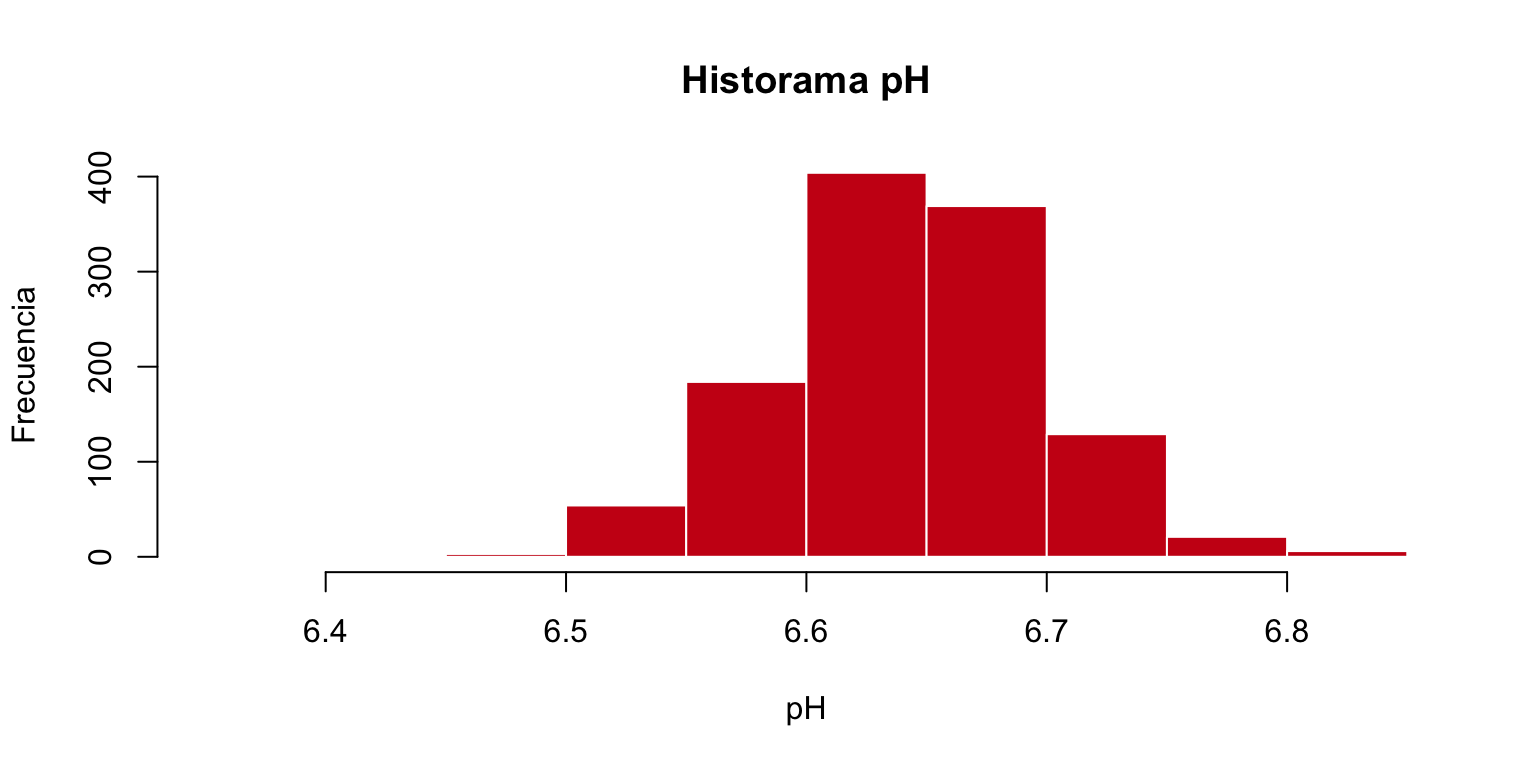
\includegraphics{91-apendices_files/figure-latex/unnamed-chunk-10-1.pdf}

\hypertarget{distribuciuxf3n-gamma}{%
\subsubsection{Distribución Gamma}\label{distribuciuxf3n-gamma}}

La distribución Gamma se utiliza, entre otros, para modelizar tiempos de
espera hasta que suceden \(\alpha\) eventos en un proceso de Poisson. De
hecho, en inferencia bayesiana gamma es la distribución a priori de la
distribución de Poisson.

\[X \sim \mathit{Ga}(a, b)\]

\textbf{Función de densidad}

\[f(x) =
\begin{cases}
\frac{b^a}{\Gamma(a)}x^{a-1}{e}^{-bx} & \text{si } 0 < x < \infty\\
0 & \text{resto }
\end{cases}\]

\textbf{Características}

\begin{itemize}
\tightlist
\item
  Esperanza: \(E[X] = \frac{a}{b}\)
\item
  Varianza: \(\mathit{Var}[X] = \frac{a}{b^2}\)
\item
  \$\Gamma(\alpha) = \int\_0\textsuperscript{\infty x}\{\alpha -1\}
  e\^{}\{-x\} dx \$
\item
  La exponencial es un caso particular
\end{itemize}

\textbf{Código}

\begin{Shaded}
\begin{Highlighting}[]
\NormalTok{migamma }\OtherTok{\textless{}{-}} \ControlFlowTok{function}\NormalTok{(x, a) }\FunctionTok{dgamma}\NormalTok{(x, a, }\DecValTok{2}\NormalTok{)}
\FunctionTok{curve}\NormalTok{(}\FunctionTok{migamma}\NormalTok{(x, }\DecValTok{1}\NormalTok{), }\AttributeTok{lwd =} \DecValTok{2}\NormalTok{, }\AttributeTok{xlim =} \FunctionTok{c}\NormalTok{(}\DecValTok{0}\NormalTok{,}\DecValTok{10}\NormalTok{), }
      \AttributeTok{main =} \StringTok{"Distribución Gamma b = 2"}\NormalTok{)}
\FunctionTok{curve}\NormalTok{(}\FunctionTok{migamma}\NormalTok{(x, }\DecValTok{2}\NormalTok{), }\AttributeTok{lwd =} \DecValTok{2}\NormalTok{, }\AttributeTok{add =} \ConstantTok{TRUE}\NormalTok{, }\AttributeTok{lty =} \DecValTok{2}\NormalTok{)}
\FunctionTok{curve}\NormalTok{(}\FunctionTok{migamma}\NormalTok{(x, }\DecValTok{4}\NormalTok{), }\AttributeTok{lwd =} \DecValTok{2}\NormalTok{, }\AttributeTok{add =} \ConstantTok{TRUE}\NormalTok{, }\AttributeTok{lty =} \DecValTok{3}\NormalTok{)}
\FunctionTok{legend}\NormalTok{(}\AttributeTok{x =} \DecValTok{6}\NormalTok{, }\AttributeTok{y =} \DecValTok{2}\NormalTok{, }\FunctionTok{c}\NormalTok{(}\StringTok{"a = 1"}\NormalTok{, }\StringTok{"a = 2"}\NormalTok{, }\StringTok{"a = 4"}\NormalTok{), }\AttributeTok{lty =} \DecValTok{1}\SpecialCharTok{:}\DecValTok{3}\NormalTok{)}
\end{Highlighting}
\end{Shaded}

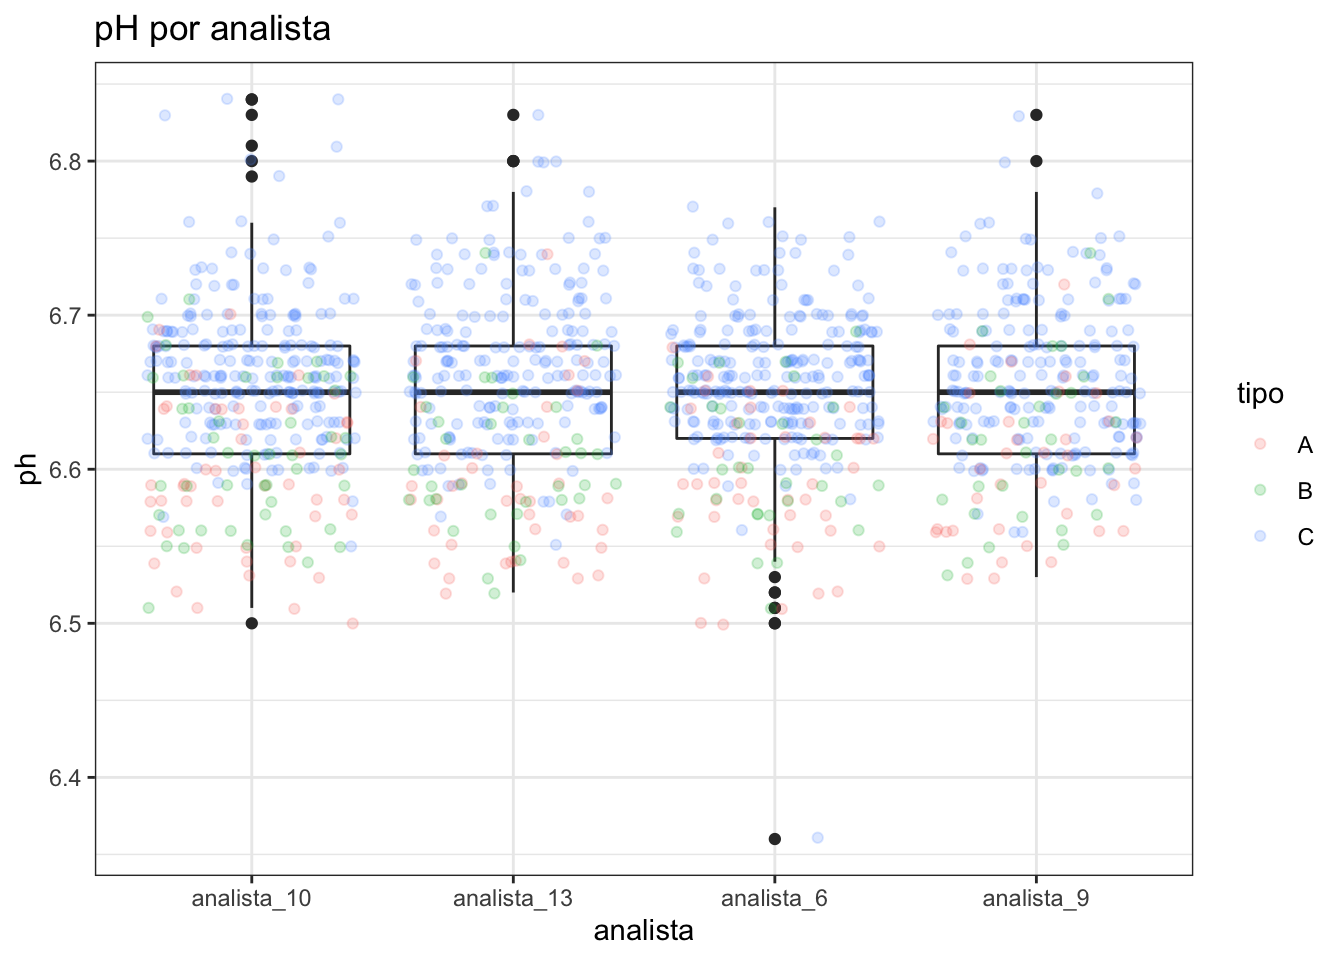
\includegraphics{91-apendices_files/figure-latex/unnamed-chunk-11-1.pdf}

\hypertarget{distribuciuxf3n-de-weibull}{%
\subsubsection{Distribución de
Weibull}\label{distribuciuxf3n-de-weibull}}

La distribución Gamma presenta algunos inconventientes al modelizar
tiempos de vida, y por eso algunas veces se prefiere la distribución de
Weibull, que básicamente sirve para lo mismo. Véase \cite{ugarte2015}
para los detalles.

\[X \sim \mathit{We}(a, b) \]

\textbf{Función de densidad} \[f(x) =
\begin{cases}
\frac{a}{b}\left (\frac{x}{b} \right)^{a-1}e^{-(x/b)^a} & \text{si } x > 0\\
0 & \text{resto }
\end{cases}\]

\textbf{Características}

\begin{itemize}
\tightlist
\item
  Esperanza: \(E[X] =b \Gamma\left (1 + \frac{1}{a} \right )\)
\item
  Varianza:
  \(\mathit{Var}[X] = b^2 \left ( \Gamma \left (  1 + \frac{2}{a} \right  )  - \left ( \Gamma \left (1 + \frac{2}{a} \right ) \right )^2 \right )\)
\end{itemize}

\textbf{Código}

\begin{Shaded}
\begin{Highlighting}[]
\NormalTok{miweibull }\OtherTok{\textless{}{-}} \ControlFlowTok{function}\NormalTok{(x, a) }\FunctionTok{dweibull}\NormalTok{(x, a, }\DecValTok{2}\NormalTok{)}
\FunctionTok{curve}\NormalTok{(}\FunctionTok{miweibull}\NormalTok{(x, }\DecValTok{1}\NormalTok{), }\AttributeTok{lwd =} \DecValTok{2}\NormalTok{, }\AttributeTok{xlim =} \FunctionTok{c}\NormalTok{(}\DecValTok{0}\NormalTok{,}\DecValTok{5}\NormalTok{), }
      \AttributeTok{ylim =} \FunctionTok{c}\NormalTok{(}\DecValTok{0}\NormalTok{, }\DecValTok{1}\NormalTok{),}
      \AttributeTok{main =} \StringTok{"Distribución Weibull b = 2"}\NormalTok{)}
\FunctionTok{curve}\NormalTok{(}\FunctionTok{miweibull}\NormalTok{(x, }\DecValTok{2}\NormalTok{), }\AttributeTok{lwd =} \DecValTok{2}\NormalTok{, }\AttributeTok{add =} \ConstantTok{TRUE}\NormalTok{, }\AttributeTok{lty =} \DecValTok{2}\NormalTok{)}
\FunctionTok{curve}\NormalTok{(}\FunctionTok{miweibull}\NormalTok{(x, }\DecValTok{5}\NormalTok{), }\AttributeTok{lwd =} \DecValTok{2}\NormalTok{, }\AttributeTok{add =} \ConstantTok{TRUE}\NormalTok{, }\AttributeTok{lty =} \DecValTok{3}\NormalTok{)}
\FunctionTok{legend}\NormalTok{(}\AttributeTok{x =} \DecValTok{4}\NormalTok{, }\AttributeTok{y =} \DecValTok{1}\NormalTok{, }\FunctionTok{c}\NormalTok{(}\StringTok{"a = 1"}\NormalTok{, }\StringTok{"a = 2"}\NormalTok{, }\StringTok{"a = 5"}\NormalTok{), }\AttributeTok{lty =} \DecValTok{1}\SpecialCharTok{:}\DecValTok{3}\NormalTok{)}
\end{Highlighting}
\end{Shaded}

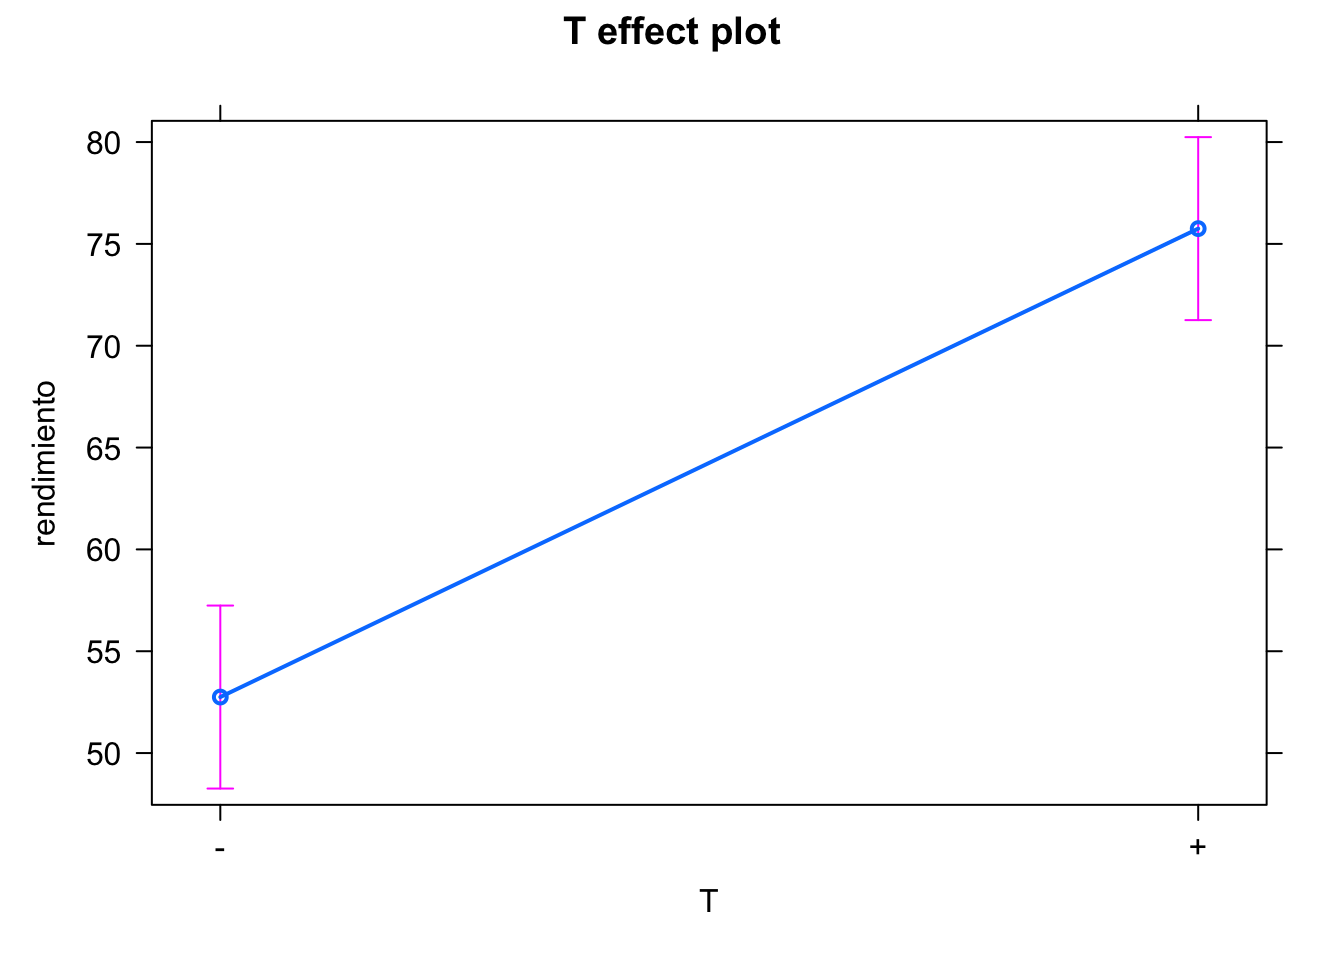
\includegraphics{91-apendices_files/figure-latex/unnamed-chunk-12-1.pdf}

\hypertarget{modelos-de-distribuciuxf3n-de-probabilidad-multivariantes}{%
\subsection{Modelos de distribución de probabilidad
multivariantes}\label{modelos-de-distribuciuxf3n-de-probabilidad-multivariantes}}

\hypertarget{modelos-de-distribuciuxf3n-de-probabilidad-relacionadas-con-la-normal}{%
\subsection{Modelos de distribución de probabilidad relacionadas con la
normal}\label{modelos-de-distribuciuxf3n-de-probabilidad-relacionadas-con-la-normal}}

\hypertarget{simulaciuxf3n-de-variables-aleatorias}{%
\subsection{Simulación de variables
aleatorias}\label{simulaciuxf3n-de-variables-aleatorias}}

\(U(0;\; 1)\): Generador de probabilidades aleatorias. Dada cualquier
función de distribución \(F\), se pueden generar valores de esa VA
obteniendo \(F^{-1}(U(0;\; 1))\)

\hypertarget{demostraciones}{%
\section{Demostraciones}\label{demostraciones}}

Em este apéndice se incluyen aquellas demostraciones de teoremas y
propiedades no incluidas en los capítulos para mantener el carácter
práctico del mismo.

\hypertarget{variable-aleatoria-discreta}{%
\subsection{Variable aleatoria
discreta}\label{variable-aleatoria-discreta}}

\hypertarget{funciuxf3n-de-probabilidad}{%
\subsubsection{Función de
probabilidad}\label{funciuxf3n-de-probabilidad}}

\hypertarget{esperanza}{%
\subsubsection{Esperanza}\label{esperanza}}

\hypertarget{varianza}{%
\subsubsection{Varianza}\label{varianza}}

\hypertarget{creditos}{%
\section{Créditos}\label{creditos}}

Los gráficos y diagramas generados son creación y propiedad del autor,
salvo que se indique lo contrario. Su licencia de uso es la misma que la
del resto de la obra, véase el Prefacio.

La
\href{https://pixabay.com/es/illustrations/fondo-abstracto-l\%C3\%ADnea-ilustración-2462436/}{imagen
de la portada} es de dominio público, obtenida en
\href{https://pixabay.com/es/}{pixabay.com}, gracias al usuario
\href{https://pixabay.com/es/users/manuchi-1728328/}{Manuchi}.

Las imágenes de tipo \emph{clipart} usadas en esta obra y las
fotografías no atribuidas pertenecen al dominio público gracias a
\href{http://www.openclipart.org}{openclipart.org},
\href{https://unsplash.com}{unplash.com} o
\href{https://pixabay.com/es/}{pixabay.com}.

The \href{https://www.r-project.org/logo/}{R logo} is (c) 2016 The R
Foundation.

\end{document}
